\documentclass{article}


\usepackage{authblk}
\usepackage{graphicx}
% if you need to pass options to natbib, use, e.g.:
%     \PassOptionsToPackage{numbers, compress}{natbib}
% before loading neurips_2022
\usepackage{subfigure}
\usepackage{blindtext}
\usepackage{tikz}
\usepackage{wrapfig}
\usetikzlibrary{positioning}

\usetikzlibrary{shapes,arrows}
% ready for submission
\usepackage[export]{adjustbox}

% to compile a preprint version, e.g., for submission to arXiv, add add the
% [preprint] option:
%     \usepackage[preprint]{neurips_2022}


% to compile a camera-ready version, add the [final] option, e.g.:
%     \usepackage[final]{neurips_2022}


% to avoid loading the natbib package, add option nonatbib:
%    \usepackage[nonatbib]{neurips_2022}


\usepackage[utf8]{inputenc} % allow utf-8 input
\usepackage[T1]{fontenc}    % use 8-bit T1 fonts
\usepackage{hyperref}       % hyperlinks
\usepackage{url}            % simple URL typesetting
\usepackage{booktabs}       % professional-quality tables
\usepackage{amsfonts}       % blackboard math symbols
\usepackage{nicefrac}       % compact symbols for 1/2, etc.
\usepackage{microtype}      % microtypography
\usepackage{xcolor}         % colors



\usepackage[final]{neurips_2023}


% to compile a preprint version, e.g., for submission to arXiv, add add the
% [preprint] option:
%     \usepackage[preprint]{neurips_2023}


% to compile a camera-ready version, add the [final] option, e.g.:
%     \usepackage[final]{neurips_2023}


% to avoid loading the natbib package, add option nonatbib:
%    \usepackage[nonatbib]{neurips_2023}


\usepackage[utf8]{inputenc} % allow utf-8 input
\usepackage[T1]{fontenc}    % use 8-bit T1 fonts
\usepackage{hyperref}       % hyperlinks
\usepackage{url}            % simple URL typesetting
\usepackage{booktabs}       % professional-quality tables
\usepackage{amsfonts}       % blackboard math symbols
\usepackage{nicefrac}       % compact symbols for 1/2, etc.
\usepackage{microtype}      % microtypography
\usepackage{xcolor}         % colors


\title{Formatting Instructions For NeurIPS 2023}
\title{LinkedGuard: Safeguarding LinkedIn Privacy by Identifying Authentic Companies, and Scraping Resumes Accordingly}


% The \author macro works with any number of authors. There are two commands
% used to separate the names and addresses of multiple authors: \And and \AND.
%
% Using \And between authors leaves it to LaTeX to determine where to break the
% lines. Using \AND forces a line break at that point. So, if LaTeX puts 3 of 4
% authors names on the first line, and the last on the second line, try using
% \AND instead of \And before the third author name.








\author{%

\textbf{Aydin Ayanzadeh}$^1$ \quad \textbf{Hrudaya Jinna}$^2$ \quad \textbf{Kiran Reddy}$^3$ \quad \textbf{An Tran}$^4$\\
\texttt{University of Maryland Baltimore County}\\


\texttt{\{RI99539,hrudayj1,aydina1,atran9\}@umbc.edu}\\

}

\begin{document}
\nolinenumbers
\maketitle


\begin{abstract}
The problem of fake companies on the LinkedIn platform posting job listings for personal information collection and identity theft, as well as a data breach where the fake profile companies obtained user information from the resumes. To combat these issues, we have created LinkedGuard, an approach to safeguarding LinkedIn privacy. Our project is divided into two parts, the first part of the project is to find out the legitimacy of the company and predict the risk label using Machine Learning. The second part of the project is the scrapper part, wherein we scrape the resume based on risk label prediction for each company. In the ML part, we have used the Decision Trees algorithm to predict whether the company is real or fake. Here, we applied a function for generating the risk level for each company based on the features which belong to our datasets. After generating the risk level, we employed a multi-classification model with machine algorithms to predict the company's risk level. Moreover, to solve the imbalanced challenge of the dataset, we applied an over-sampling approach entitled SMOTE to synthesize the data based on the class with a minority than other classes. By employing SMOTE, the model's accuracy increased on each class efficiently, and it led to the model becoming more generalized on the classes which have a lower frequency. To prove the model's robustness in our dataset, we also applied k-fold cross-validation to show the model's performance on different folds of the dataset.


This risk label is then inputted into the scrapper, and the scrapper scrapes the resume. We have written a policy for allocating the risk factors to each element in the resume and we have written a policy of what fields to be scrapped in the resume and why. We looked into many resources and found some factors which contribute to the legitimacy of the company. We sent a survey to the class and neighborhood. This survey had questions and factors which relate to the legitimacy of the company. Regarding the qualitative analysis of the determined features, we prepared a survey and 45 people who filled out the survey form were in different age groups and tended to use LinkedIn for their goals. We carefully looked into the survey results and examined the results they provided. After a thorough quantitative and qualitative investigation of the results, we have extracted 11 features from it. These features were used in a dataset for predicting the company's legitimacy on LinkedIn using Machine Learning.

\section*{Keywords:}
Machine Learning, Decision Trees, risk prediction, company legitimacy, resume scraper, survey analysis, LinkedIn, data privacy, fake companies.
\end{abstract}


\section{Introduction}
Detecting fake companies on LinkedIn is important because it helps to protect users from scams and identity theft. Scammers can easily access and gather personal and sensitive user information, and users are often less aware and least concerned about security settings. Fake profiles can have an adverse effect on the trustworthiness of the network as a whole and can represent significant costs in time and effort in building a connection based on fake information.

We recently encountered a situation where a company posted a job opening for software developers. During the final stage of the application process, the recruitment team asked the candidate to write a review of the products they sold and give the ratings. However, later the candidate got to know that it was a fake company. Job openings for software developers typically do not involve the task of reviewing and providing ratings for a company's products.
This might not look like a major issue, but be aware that a few companies tend to go further in scam and ask the candidate to pay for the courses they offer as a part of the recruitment process.

Most of the time, we provide our resumes to fake companies, and these fake companies steal our information and use it to commit fraud. 
There is even a data breach instance where LinkedIn has already faced data breaches. One of the fake profile companies obtained information about users from resumes sent to them. 

In 2019, a fake company called "Asheville Matrix LLC" posted job listings for various positions on LinkedIn. The scammers conducted interviews and even extended offers to unsuspecting candidates. However, the company did not exist, and the scammers attempted to collect personal information and potentially engage in identity theft.

We had seen an instance in one of the user’s LinkedIn posts where he had a screenshot of the mail that he received from xyz company. The email states that he was selected for a job interview. The message says that they obtained or her resume from Indeed.com. But the actual fact is, that particular candidate never applied to this job from Indeed.com. The sentence formation in the data provided in the mail was also not that good.  The email reference of the recruiter person mentioned in the mail had a generic expansion for the email that is gmail.com and not company specific email.  The phone number provided was also VOIP (voice over internet protocol) based, and is "non-fixed". Using VOIP, you can get a new phone number any time you choose; difficult to investigate too.

This provided us motivation to look into companies that are not legitimate, and we wanted to build a model where it detects whether the company is real or fake. On the other hand, the most important privacy concern here is that no individual wants to give away his resume without knowing the legitimacy of the company because if in case the resume goes into the hands of fake companies, then they can do any kind of scams like sending phishing emails to a candidate or be a cause of user data breach. 

Our major goal was not to give away our resume to the company without knowing how legitimate the company was. Each company might have different levels of risks associated with it. So we decided to analyze the risk factor and predict risk for each company, and based on the risk factor, we want to scrap the original resume to showcase only a part of the resume to the companies. 

After conducting extensive research, we identified various factors that contribute to determining the legitimacy of a company. These factors were carefully documented and compiled into a survey. The survey was then distributed to individuals within our class and neighborhood as Shown in Figure\ref{fig:flowchart1}. It was encouraging to receive responses from over 45 participants, representing diverse age groups who regularly utilize LinkedIn for various purposes.

We meticulously analyzed the survey results, considering both quantitative and qualitative aspects. Through this comprehensive investigation, we identified 11 key features that were derived from the survey data. These features were incorporated into a dataset to train a Machine Learning model for predicting the legitimacy of companies on LinkedIn as shown in Figure \ref{fig:flowchart1}.

Now utilizing these 11 features, we created a dataset. The dataset contains 11 features, and we have added a company name column to it. So, in total, now the dataset has 12 features.  We utilized this dataset to create a model in ML which predicts whether the company is real or fake. We found the precision-recall accuracy and F1 score for all our implemented algorithms. When a feature input is fed to the model, the model predicts whether the company is real or fake. 
We have assigned a risk label to every company, using a scale ranging from 0 to 5. A risk label of 0 indicates that the company carries no associated risk, while a label of 5 indicates that the company is considered to be at a high level of risk.


\begin{figure}
\centering
\begin{tikzpicture}[node distance=4cm, scale=0.9, transform shape]
    
    \tikzstyle{block} = [rectangle, draw, text width=6em, text centered, minimum height=4em]
    \tikzstyle{line} = [draw, -latex]
    
    \node [block] (input) {Conducted online survey for knowing the factors that affect the legitimacy of the company};
    \node [block, right of=input] (preprocessing) {Based on survey, selected 11 factors};
    \node [block, right of=preprocessing] (eda) {Created dataset using these 11 factors};
    \node [block, right of=eda] (features) {Built ML code to determine the legitimacy of the company};
    \node [block, below of=features] (divide) {Added risk label ranging from 0 to 5 for each company};
    \node [block, left of=divide] (model) {Predicted risk label};
    \node [block, left of=model] (evaluate) {Used risk label as input to the scrapper};
    \node [block, left of=evaluate] (predict) {Scrapper scrapes the resume based on risk label};   
    
    % Draw edges
    \path [line] (input) -- (preprocessing);
    \path [line] (preprocessing) -- (eda);
    \path [line] (eda) -- (features);
    \path [line] (features) -- (divide);
    \path [line] (divide) -- (model);
    \path [line] (model) -- (evaluate);
    \path [line] (evaluate) -- (predict);
    
    % Add title
    \node [above] at (current bounding box.north) 
\end{tikzpicture}
\caption{High level flowchart of the project}
\label{fig:flowchart1}
\end{figure}


\section{Background and Related work}
A paper was written by Pandya et al.[1] on "Detection of Deceptive Accounts Using Machine Learning Algorithm and Deep Neural Network" in 2020. In this paper, the authors tested the efficiency of machine learning techniques and deep neural networks in detecting fake accounts through their analysis of a dataset that includes both authentic and fake accounts. The results showed that deep neural networks, specifically convolutional neural networks (CNN), outperformed classical machine learning techniques in terms of accuracy.

A paper written by Sahoo et al.[2] on "Identification of Malicious Accounts on Facebook" in 2019 focused on classifying fraudulent and legitimate Facebook profiles using various machine learning algorithms. The authors tested classifiers such as decision trees, random forests, SVM, and KNN, and evaluated their effectiveness using metrics such as accuracy, precision, recall, and F1-score. Their methodology demonstrated reliable and precise identification of rogue accounts in a dataset comprising both account types.

The work of Khaled et al.[3] in 2018 on "Detecting Fake Accounts on Social Media" served as a reference. The authors gathered data from user profiles, posts, interactions, public blacklists, and user reports to identify distinct patterns of fake accounts. They employed machine learning algorithms such as decision trees, random forest, logistic regression, and SVM for account classification, evaluating their performance using common evaluation criteria.

Adikari and Dutta's[4] paper in 2020 on "Identifying Fake Profiles in LinkedIn" addressed the problem of detecting fake profiles on LinkedIn. The authors proposed a data mining strategy to detect fraudulent profiles based on limited profile information. Their method achieved an accuracy of 87\% and a True Negative Rate of 94\%, demonstrating its effectiveness even with limited data. This study focused on detecting fake profiles rather than fake companies on LinkedIn.

After thoroughly examining these papers, we found that our project of utilizing a Machine Learning model[5] to detect the legitimacy of companies on LinkedIn incorporates a unique and novel aspect, the implementation of a scrapper. Previous research did not specifically focus on identifying fake companies on LinkedIn or integrating a scraper with Machine Learning. Therefore, our project marks the first-time implementation of Machine Learning and a scrapper to determine company legitimacy and extract relevant information from resumes based on risk labels. Unlike the paper by Adikari, our work specifically addresses the detection of fake companies on LinkedIn, making it a novel contribution in this domain.



\section{Dataset}

We have sent a survey link to both the class and the neighborhood. This survey aimed to gather information regarding the legitimacy of companies on LinkedIn. The survey included multiple questions that helped us identify the factors contributing to determining whether a company is real or fake. We received 45 responses from individuals of various age groups who use LinkedIn. After conducting a qualitative analysis of the survey data, we identified potential new features that could be added. Upon thorough examination of the survey results, we concluded to consider the top 11 features. Each feature will be assigned a value of 1 or 0. After considering all 11 features, we have decided to construct a dataset. We need a list of companies to create this dataset. The dataset now includes a column for company names. Therefore, the 12 features (we excluded the company name from our evaluation and we counted it as datapoint ID) are as follows:  

\begin{enumerate}
\item Company Name (Excluded in our machine learning analysis)
\item LinkedIn Followers > 1000
\item Profile Picture
\item Responsive Website
\item	Staff Count > 1000
\item	Staff Premium Accounts
\item	Summary Section
\item	Verified Address
\item	Published Articles
\item	Requests Sensitive Info
\item	Legitimate Email
\item	LinkedIn Recommendations
\end{enumerate}


Fortunately, IBM and TCS have provided us with a comprehensive list of both fake and real companies. From this list, we have selected companies to include in our dataset, taking into account their classification as fake or real. We have added a new column to the dataset specifically indicating whether a company is fake or real. This column, denoted as "Company Real or Fake," with values of 1 or 0, serves as the 13th feature in our dataset. After doing the qualitative analysis by doing a survey, we extracted the top-5 most important factors amount the 11 factors we have in our dataset as features. The list of top-5 features is shown in Table \ref{top-5}.

To ensure the accuracy of each feature value, we manually verified the data for a total of 100 companies. For each cell, we filled in the corresponding values for 50 real companies and 50 fake companies. Subsequently, utilizing the available real and fake company lists, we synthesized the data for the remaining cells based on the classification of the respective companies. As a result, the dataset now comprises 801 rows, encompassing the collected information.

\begin{figure}
\centering
\begin{tikzpicture}[node distance=4cm, scale=0.9, transform shape]
    
    \tikzstyle{block} = [rectangle, draw, text width=6em, text centered, minimum height=4em]
    \tikzstyle{line} = [draw, -latex]
    
    \node [block] (input) {Importing DataSet};
    \node [block, right of=input] (preprocessing) {Performing Dta preprocessing};
    \node [block, right of=preprocessing] (eda) {EDA};
    \node [block, right of=eda] (features) {Feature Selection};
    \node [block, below of=features] (divide) {Dividing Training and Testing Datasets};
    \node [block, left of=divide] (model) {ML model Implementation};
    \node [block, left of=model] (evaluate) {Evaluate Model, (Precision, Recall,F1 Score, Accuracy};
    \node [block, left of=evaluate] (predict) {Provide Input to Model and Predict Target Variable};   
    
    % Draw edges
    \path [line] (input) -- (preprocessing);
    \path [line] (preprocessing) -- (eda);
    \path [line] (eda) -- (features);
    \path [line] (features) -- (divide);
    \path [line] (divide) -- (model);
    \path [line] (model) -- (evaluate);
    \path [line] (evaluate) -- (predict);
    
    % Add title
    \node [above] at (current bounding box.north) 
\end{tikzpicture}
\caption{Steps for finding out the legitimacy of the company}
\label{fig:flt}
\end{figure}




\begin{table}[h]

\begin{center}

\caption{List of Top-5 factors obtained from the dataset features.}
\label{top-5}
\begin{tabular}{|c|}
\hline

Legitimate Email \\ \hline
Profile picture  \\ \hline
Responsive website   \\ \hline
verified Address   \\ \hline
Request Sensitive Info \\ \hline


\end{tabular}
\end{center}
\end{table}


\begin{figure}[h]%
\centering
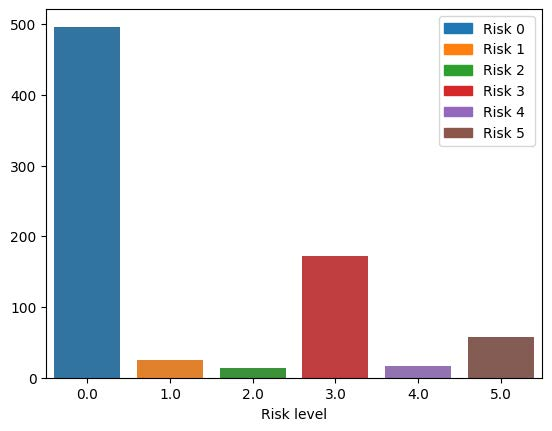
\includegraphics[width=0.7\textwidth]{imbalanced.jpg}
\caption{The frequency of data points for each risk level class.}\label{dist}
\end{figure}



\section{Design and Analysis}

In this section, we explained the machine learning method which we employed in our datasets. All subsections including Model selection, Imbalanced data and k-fold cross-validations, and experimental results of this section are covered in this section. 


\subsubsection{Model Selection}

Model selection in machine learning is choosing the most appropriate algorithm or model for a given problem. It involves evaluating and comparing different models based on their performance and selecting the one that best meets the requirements and objectives of the task at hand. In this project, we applied three well-known applications, including Support Vector Machine, Decision Tree, and K-Nearest Neighbor(KNN) approaches to evaluate our model's performance. In case of model selection, we follow up the structured machine learning application to predict the risk level and company legitimacy (Real or Fake). Firstly we define the problem we are trying to solve and start to determine the requirement for our classification task. 

Firstly, the initial step involves importing the dataset into either a Jupyter Notebook or Google Colab. The subsequent step entails verifying the presence of null values. As our dataset contained minimal null values, we eliminated rows with null values. The subsequent step in data preprocessing involves examining for duplicate values. Since our dataset had no null values, no modifications were made. Since the majority of the data consists of numerical values, this aspect was satisfactory. However, the "Company Name" column contained company names represented by alphabets. Therefore, we employed Label encoding to convert the data in that column into a numerical form. The data must undergo preprocessing and cleaning procedures to ensure that it is in an appropriate format for modeling purposes. 

Following that, we proceeded with exploratory data analysis (EDA), wherein we analyzed the data by creating several graphs to gain further insights. Finally, for feature selection, we utilized a heatmap to determine the correlation between each feature in the dataset. We then performed a correlation analysis of all the features with the target feature, which is "Company Real or Fake." We sorted the features in descending order to identify the most highly correlated ones, as shown in Figure \ref{corel1}. However, since this analysis is experimental in nature, relying solely on a few features with high correlation is not advisable. Consequently, we decided to consider all features when predicting the legitimacy of a company.

\begin{figure}[h] 
\centering
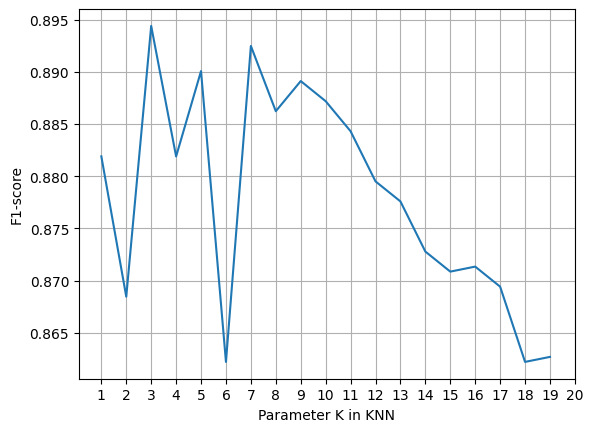
\includegraphics[width=0.8\textwidth]{Knn-plot.png}
\caption{The f1-score value for different k-value in KNN model.} \label{knn}
\end{figure}

 Split the data: Divide the available data into training, validation, and test sets. The training set is used to train the models, and the test set is used to assess the final performance of the selected model. In our experiments, we employed 30 percent of datasets for the test set and used the rest for training the models. 
 
 
 Evaluation metrics are employed to evaluate and compare the performance of different models, and choosing evaluation metrics for machine learning is problem-dependent. In this project, we, employed well-known classification metrics, including accuracy, precision, recall, and F1-score, to evaluate the model's performance on different models. The formula of Precision, Recall, and F1 score is presented in Equation\ref{eq: precision}-\ref{eq:dice}, respectively, where P denotes the precision, R denotes the Recall, and $n_{tp}$, $n_{fp}$, and $n_{fn}$ indicate the numbers of true positives, false positives, and false negatives, respectively.




 

 \begin{equation}\label{eq: precision}
Precision= \frac{n_{tp}}{ n_{fp}+ n_{tp}}
\end{equation}

\begin{equation}\label{eq: recall}
Recall=\frac{n_{tp}}{ n_{fn}+n_{tp}}
\end{equation}



\begin{equation}\label{eq:dice}
F1 score =\frac{2 |PxR|}{ |P| + |R| }
\end{equation}


 
 
 
 In case of training the model, we also applied the hyper-parameter optimization to find the best parameters in our employed model. For instance, we put the visualization of the hyper-parameter optimization on KNN model for different K, as shown in Figure\ref{knn}. This plot shows that the best k value for the KNN model is 3, which gives the highest F1 score compared to the k value.
 









% Inputting dataset
% Performing Data Preprocessing
% Exploratory Data Analysis (EDA)
% Feature selection
% Dividing dataset into Training and Testing sets
% Implementing Machine Learning (ML) model
% Evaluating accuracy scores
% Providing input to the model for target prediction








These are the features of correlation.
\begin{figure}[h]%
\centering
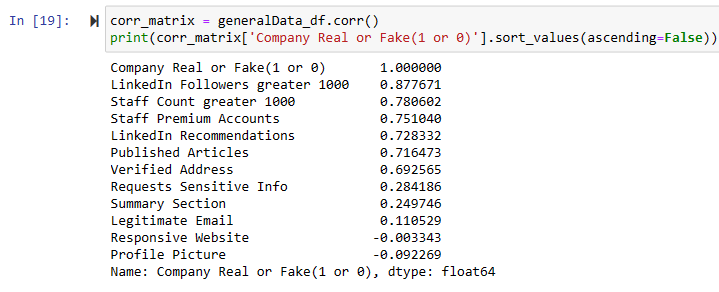
\includegraphics[width=0.9\textwidth]{corr_matrix.png}


\caption{Correlation with respect to company real or fake in descending order}\ \label{corel1}
\end{figure}


In order to predict whether a company is real or fake, our task involves a binary classification, where the prediction is either a "yes" or "no" outcome. This implies that we are distinguishing between two classes. Therefore, for this particular problem, we opted for machine learning models that fall under the classification type. Conversely, since our prediction does not involve continuous values, we did not choose regression models.

In order to predict the risk level, we also applied multi-classification models to predict the risk level in our applications. Regarding the risk level generation, we applied a regularization factor, which reward the top-5 important factors against the other features in our dataset. To solve this, we start to generate a function. for handling the range of the generated value and also controlling the level of rewards to the most important factors, we determine the $\alpha = 1.19$, based on Equation\ref{eq1}, we assume all the legitimate company Risk level 0, so we applied this function on the companies which are fake and assume $n=5 $ for the features($f_i$) for the top-5 features. After getting the risk value from Equation\ref{eq1}, we categorized the risk level based on Table\ref{range} to map the risk value to the proper risk label.

\begin{center}
    \begin{equation}   \label{eq1} 
  R=\left\{
    \begin{array}{ll}
       0, & \mbox{All legitimate companies}.\\
      \sum_{n=1}^{11} \alpha^n f_i 
& \mbox{otherwise}.  
    \end{array}
  \right. 
\end{equation}

\end{center}







To proceed with our analysis, we divided the dataset into training and testing sets as shown in Figure \ref{fig:flt}.
We initially implemented the Decision Trees algorithm. This supervised machine-learning approach is used for both classification and regression problems. It constructs a model with a tree-like structure to make decisions based on input features.

The root node, representing the complete dataset, serves as the starting point in the decision tree. The algorithm then divides the data at each node into multiple classes or minimizes overall variance (in the case of regression) based on a chosen feature. Typically, criteria such as Gini impurity or information gain are utilized to determine the most suitable feature for division.
\begin{table}[]
\begin{center}
\caption{Risk level range for categorizing the risk value.}\label{range}
\begin{tabular}{|c|c|}

\hline
 Range & Risk Level \\ \hline
 [0,5]& 5 \\ \hline
(5,7] & 4 \\ \hline
(7,9] & 3 \\ \hline
(9,10] & 2 \\ \hline
(>10) &  1\\ \hline
\end{tabular}
\end{center}
\end{table}
For this model, we calculated metrics such as Precision, Recall, F1 score, and support. The accuracy achieved by this algorithm was 95.65\% 

Having trained the model, we are now able to provide 12 feature inputs to the model, which in turn predicts whether the company is real (0) or fake (1) as shown in Figure\ref{features_fake} and Figure\ref{features_real}

\begin{figure}[h]%
\centering

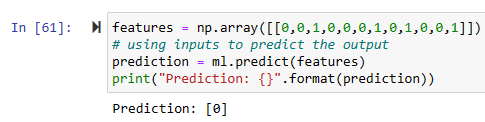
\includegraphics[width=0.9\textwidth]{features.png}
\caption{Model Predicted the company is fake}\label{features_fake}
\end{figure}


\begin{figure}[h]%
\centering

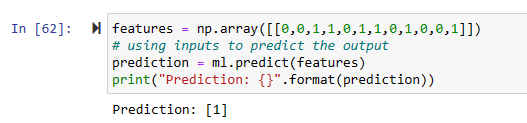
\includegraphics[width=0.9\textwidth]{pred.png}
\caption{Model predicted the company is real}\label{features_real}
\end{figure}
%\subsubsection{Imbalanced Datasets}



%\subsubsection{Over-sampling }

\subsubsection{Imbalanced Dataset}

As we explained in the prior section, the frequency of each risk label is distributed unequally. The number of data points with a risk level of 0 is more than other risk labels which cause the machine learning model to have a lower prediction accuracy. The frequency of the  datapoint for each class of risk level is shown in Figure\ref{dist} To tackle this problem, we applied an over-sampling approach which synthesizes the data points in the classes which have a minority to the other risk label. The over-sampling method which I used is Synthetic Minority Over-sampling Technique (SMOTE). SMOTE is an oversampling algorithm that addresses the issue of imbalanced classification datasets, where the representation of classification categories is unequal. The SMOTE technique generates synthetic data for the purpose of oversampling through the utilization of a k-nearest neighbor algorithm. The algorithm conducts an iterative process in which it traverses through each observation belonging to the minority class. During this process, it identifies the k nearest neighbors of each observation and subsequently chooses a random set of neighbors for the generation process. The quantity of utilized neighbors is contingent upon the level of oversampling that is necessary.
The SMOTE technique produces synthetic instances from the underrepresented class that are deemed plausible, meaning that they are situated in the feature space in proximity to the pre-existing instances from the underrepresented class.




% \subsubsection{Over-sampling }

% The Synthetic Minority Over-sampling Technique (SMOTE) is an oversampling algorithm that addresses the issue of imbalanced classification datasets, where the representation of classification categories is unequal. The SMOTE technique generates synthetic data for the purpose of oversampling through the utilization of a k-nearest neighbor algorithm. The algorithm conducts an iterative process in which it traverses through each observation belonging to the minority class. During this process, it identifies the k nearest neighbors of each observation and subsequently chooses a random set of neighbors that will be utilized in the generation process. The quantity of utilized neighbors is contingent upon the level of oversampling that is necessary.
% The SMOTE technique produces synthetic instances from the underrepresented class that are deemed plausible, meaning that they are situated in the feature space in proximity to the pre-existing instances from the underrepresented class.


We applied the SMOTE, which increased the number of data pint from 800 to 2796, which led to an increase in the number of data points to satisfy the model's robustness and completeness in the case of prediction accuracy. Based on the quantitative results which are shown in Figure \ref{wo-smote-svm}, Although the SVM's accuracy in total is around 90 percent, the model's accuracy for the class2 and class 4 is 0; it means that the model can not be trained for that classes and the main reason for this occurrence can be the low amount of labeled value for these classes. By applying the SMOTE techniques, the model's accuracy for class 2 and class 4 is increased to 85\% and 75\%,  respectively. The quantitative results for the three models after and before the over-sampling approach is shown from Figure\ref{wo-smote-svm}-\ref{knn_reppo}
Moreover, a confusion matrix is also added to show the frequency of correct and wrong predictions for each class in the applied model, and all of the determined confusion matrices are also shown from Figure \ref{conf1}-\ref{knn-conf} efficiently.

\subsection{K-fold cross validation}


K-fold cross-validation is a method for analyzing the efficacy and generalizability of a machine-learning model. The given dataset must be divided into k equally sized subgroups, or "folds," where k is a fixed integer. The model is trained and tested k times, with each fold acting as a validation set once and being used to train the remaining folds. In this project, as we mentioned in prior sessions, our dataset encountered an imbalance challenge, which we solved by SMOTE approach. We applied k-fold cross-validation to prove the model's performance and robustness on applied datasets. We also showed the results of the applied model by passing the k-fold cross-validation techniques to prove the generalizability of the model and applied approaches. The quantitative results of the three models are shown in Table\ref{k-fold1}.




\begin{table}[]
\caption{k-fold cross validation results for three employed models.}
\label{k-fold1}
\begin{center}
\begin{tabular}{|l|l|l|l|l|l|}

\hline
Model & Fold 1  &  Fold 2& Fold 3 & Fold 4 & Fold 5 \\ \hline
KNN & 0.7835  &  0.9042& 0.8218 & 0.8956 &  0.8672\\ \hline
SVM & 0.8724 &0.8436  &0.8722  & 0.8403 & 0.8521 \\ \hline
Decision Tree & 0.9144 & 0.9126 & 0.9058 & 0.9126 & 0.8941 \\ \hline

\end{tabular}
\end{center}
\end{table}



\begin{figure}[h]\label{svm-conf}
\centering
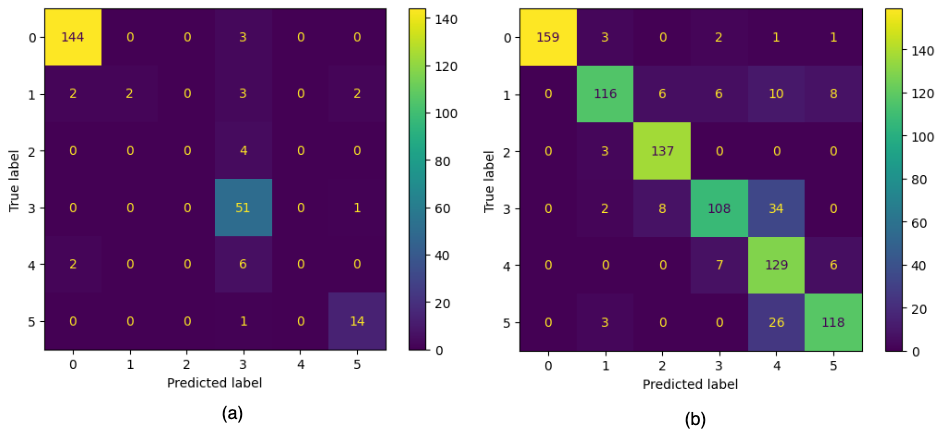
\includegraphics[width=0.9\textwidth]{SVM_confusion.png}
\caption{(a) confusion matrix before over-sampling on SVM and (b) is the confusion matrix after SMOTE technique.}\label{conf1}
\end{figure}


\begin{figure}[h]\label{tree-conf}
\centering
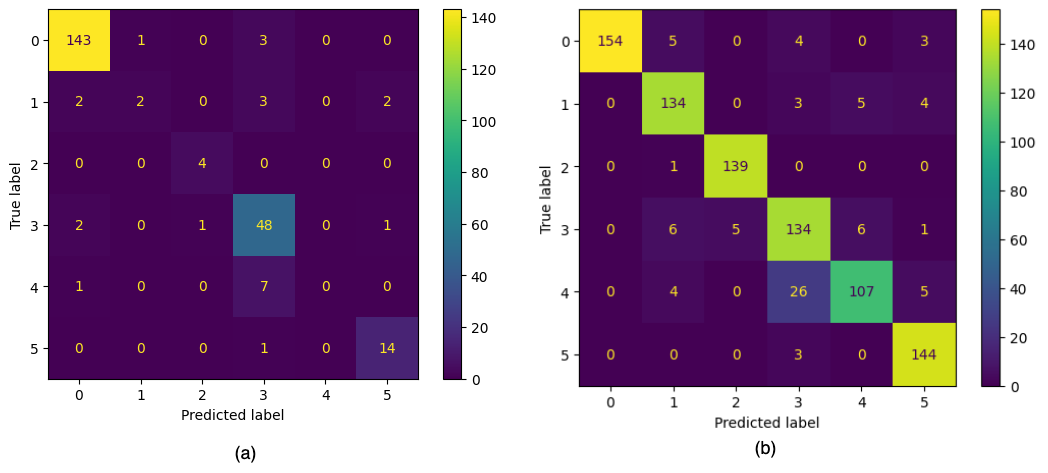
\includegraphics[width=0.9\textwidth]{tree_conf.png}
\caption{(a) confusion matrix of Decision tree before over-sampling and (b) is the confusion matrix of Decision tree after SMOTE technique.}\label{fig1}
\end{figure}



\begin{figure}[h]
\centering
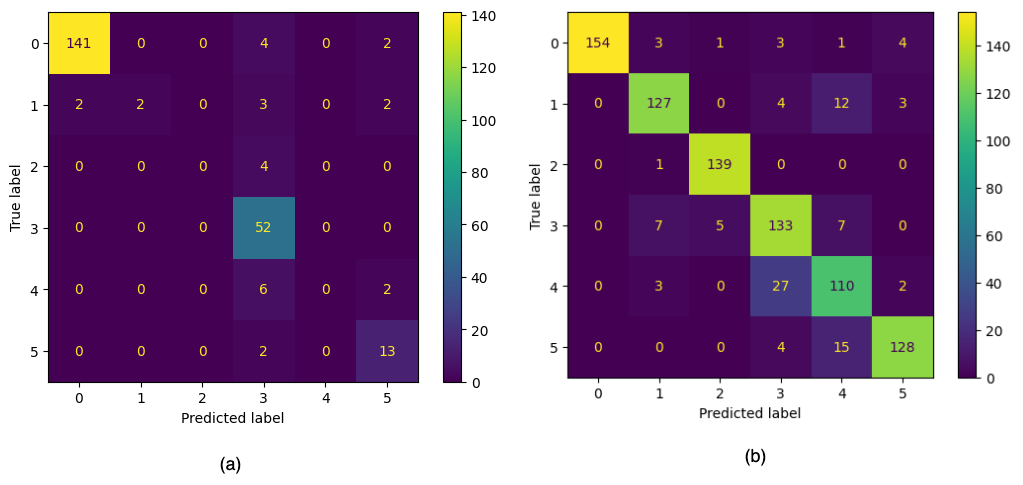
\includegraphics[width=0.9\textwidth]{KNN_conf.png}
\caption{(a) confusion matrix of KNN before over-sampling and (b) is the confusion matrix of KNN after SMOTE technique.}\label{knn-conf}
\end{figure}


\begin{figure}[h]
\centering
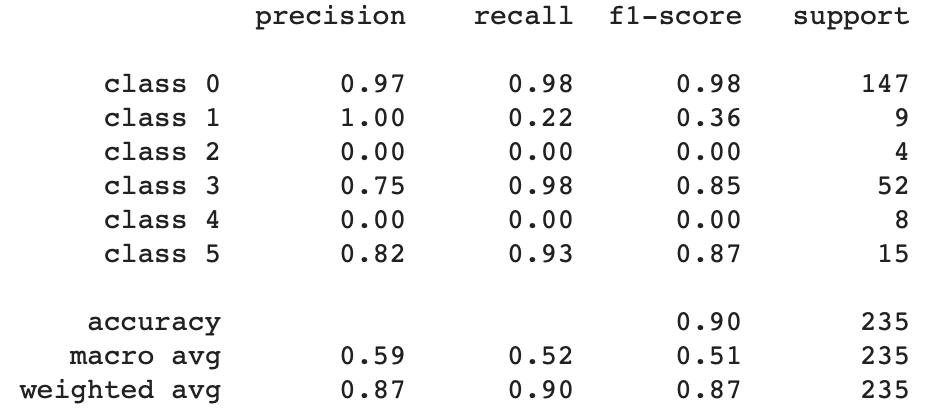
\includegraphics[width=0.8\textwidth]{SVM_b.png}
\caption{(a) The summary of the accuracy report for each class on SVM model before the implementation of SMOTE.}\label{fig1}
\label{wo-smote-svm}
\centering
\end{figure}


\begin{figure}[h]\label{smote-svm}
\centering
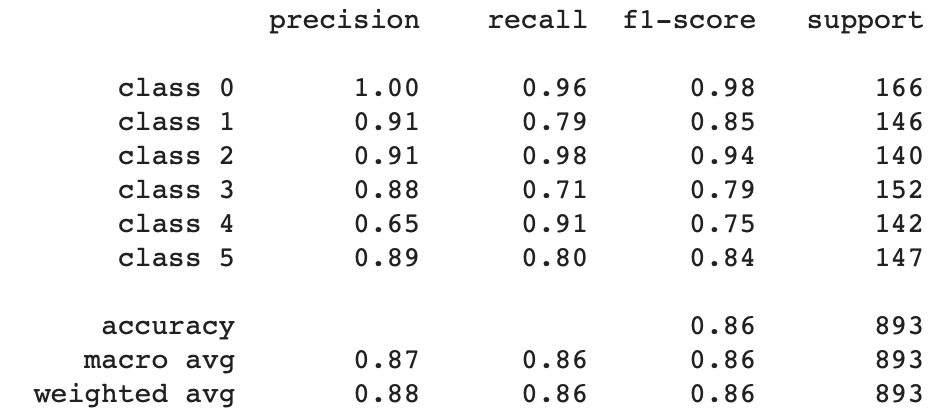
\includegraphics[width=0.8\textwidth]{sv_a.png}
\caption{(a) The summary of the accuracy report for each class on SVM model after the implementation of SMOTE.}\label{fig1}
\end{figure}




\begin{figure}[h]
\centering
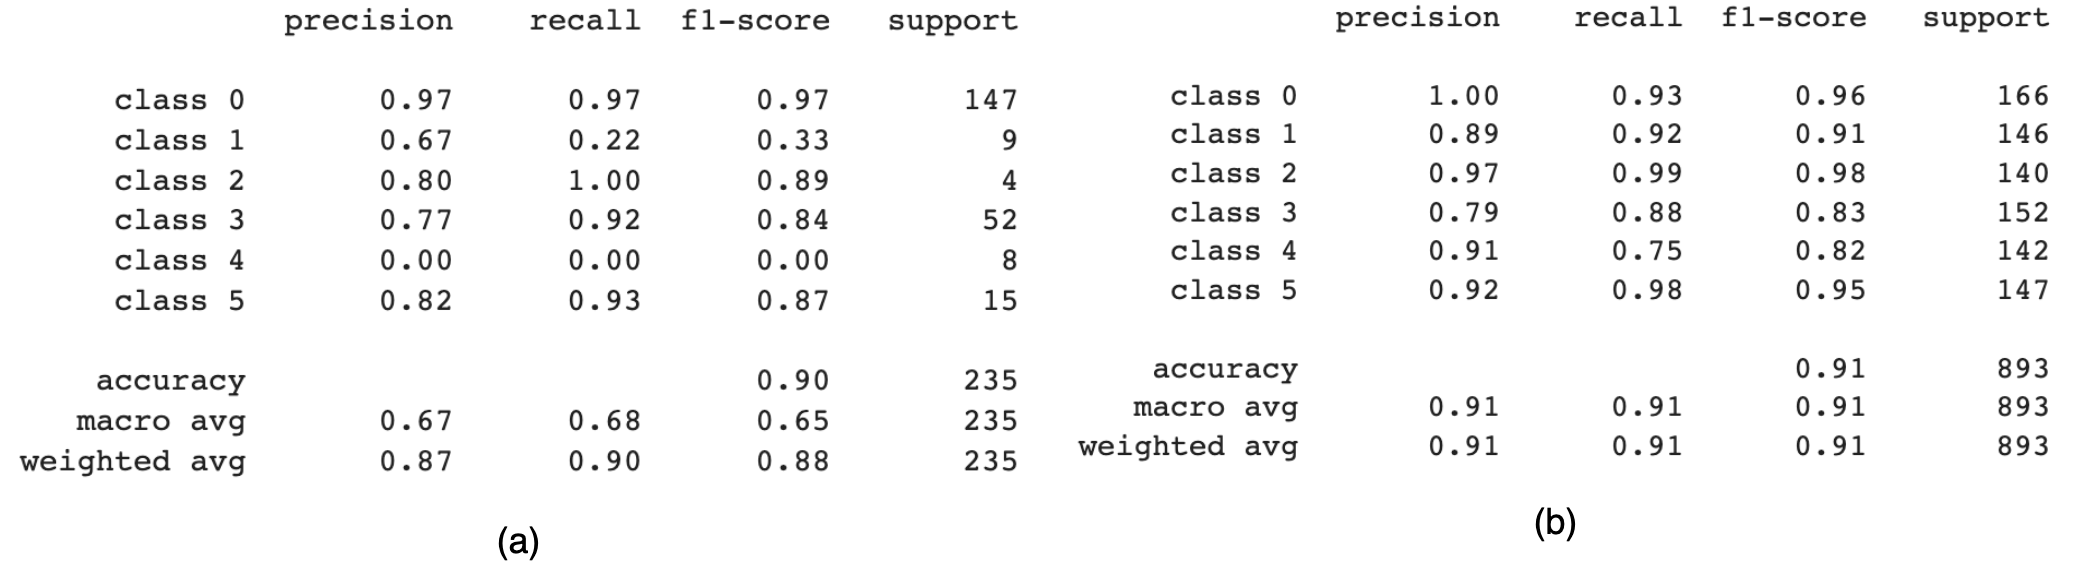
\includegraphics[width=0.98\textwidth]{ddtree.png}
\caption{(a) The summary of the accuracy report for each class on the Decision Tree model before the implementation of SMOTE and (b) is the accuracy report of Decision Tree after the SMOTE implementation.}\label{decis_reppo}
\end{figure}



\begin{figure}[h]
\centering
% \label{knn_repp}
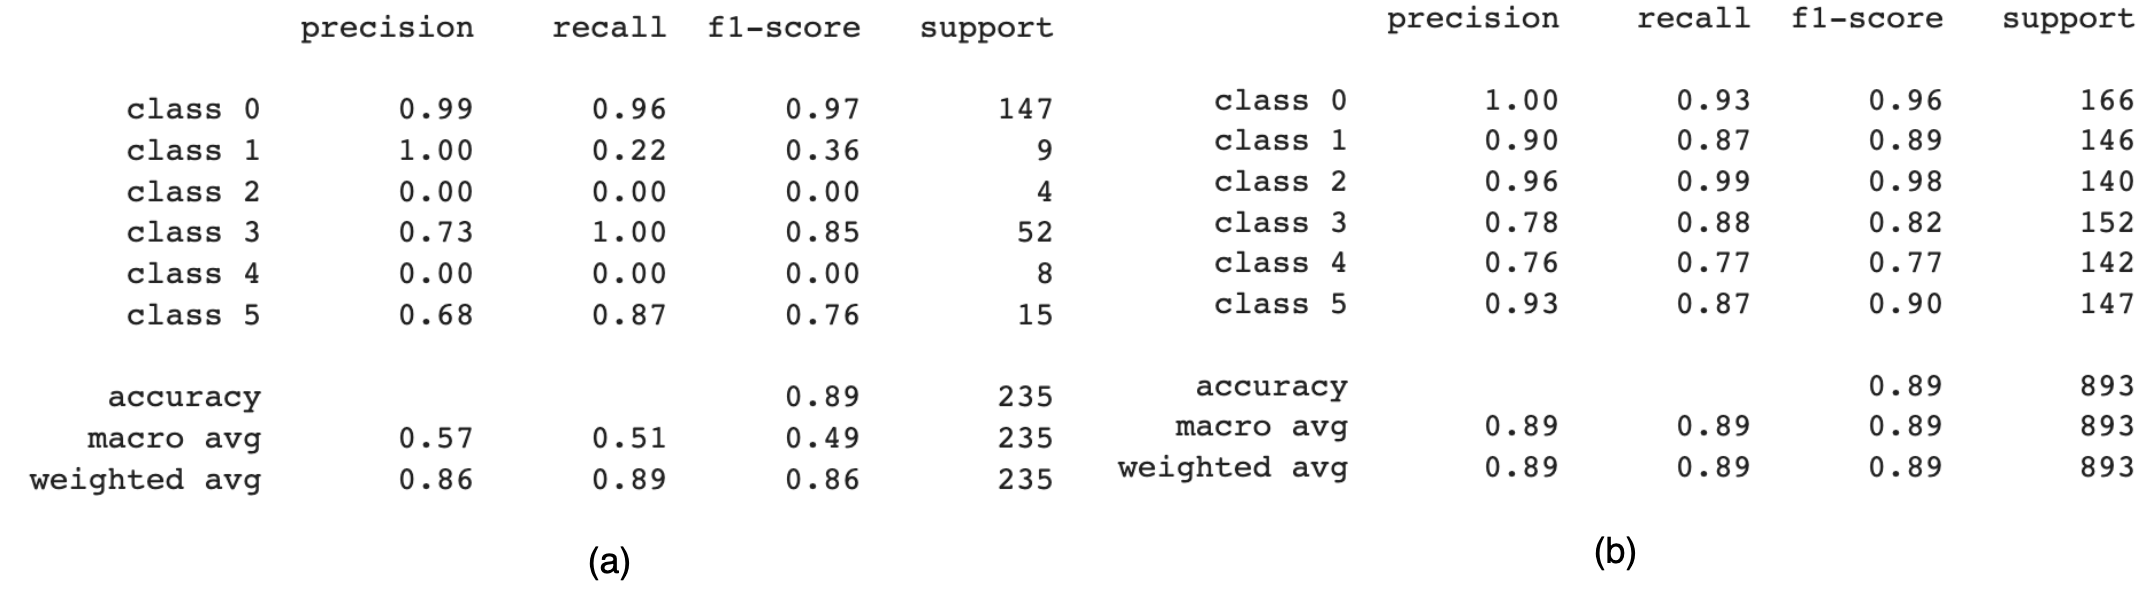
\includegraphics[width=0.99\textwidth]{knn_finalll.png}
\caption{(a) The summary of the accuracy report for each class on the KNN model before the implementation of SMOTE and (b) is the accuracy report of KNN after the SMOTE implementation.}\label{knn_reppo}
\end{figure}






% \begin{table}[]
% \begin{center}
% \begin{tabular}{|c|c|c|c|c|c|}
% \caption{The model }
% \hline
%   Model& Fold 1 & Fold 2& Fold 3 & Fold 4 & Fold 5  \\ \hline
% KNN&  0.8724 &  0.8436 & 0.8722 & 0.8403 & 0.8521\\ \hline
% KNN&   0.7835& 0.9042 & 0.8218 & 0.8756 & 0.8672\\ \hline
% Decision Tree & 0.9144 &0.9126 & 0.9058& 0.9126&0.8941\\ \hline

% \end{tabular}
% \end{center}

% \end{table}




% \begin{itemize}
%     \item  Profile picture
%     \item Responsive website
%     \item verified Address 
%     \item Request Sensitive Info
%     \item  Legitimate Email
% \end{itemize}


\section{Risk Factor Analysis}
The next step in the risk management process involves classifying the identified risk factors based on their potential impact and likelihood of occurrence. To ensure consistency and objectivity in the risk assessment process, a 0-5 scaling system is used to classify the risk factors.
The 0-5 scaling system categorizes the risk factors into six levels based on their potential impact and likelihood of occurrence. The levels are and shown in Table \ref{demo-table}:
\begin{itemize}
  \item \textbf{Level 0: No Risk} - Risk factors that are unlikely to occur or have a minimal impact if they do. No further action is required for these risk factors.
  \item \textbf{Level 1: Low Risk} - Risk factors that have a low likelihood of occurring or have minimal impact if they do. These risk factors can be monitored and managed through routine procedures.
  \item \textbf{Level 2: Moderate Risk} - Risk factors that have a moderate likelihood of occurring and could have a moderate impact if they do. These risk factors require careful monitoring and management to prevent or mitigate their impact.
  \item \textbf{Level 3: High Risk} - Risk factors that have a high likelihood of occurring and could have a significant impact if they do. These risk factors require immediate attention and proactive management to prevent or mitigate their impact.
  \item \textbf{Level 4: Very High Risk} - Risk factors that are almost certain to occur and could have severe consequences if they do. These risk factors require urgent action and special measures to prevent or mitigate their impact.
  \item \textbf{Level 5: Extreme Risk} - Risk factors that are virtually guaranteed to occur and could have catastrophic consequences if they do. These risk factors require immediate and decisive action to prevent or mitigate their impact.
\end{itemize}

\begin{table}
    \centering
    \begin{tabular}{|p{0.15\linewidth}|p{0.2\linewidth}|p{0.5\linewidth}|}
        \hline
        \textbf{Levels} & \textbf{Risk} & \textbf{Description}\\
        \hline
        Level 0 & No Risk & Have a minimal impact. No further action is required.\\
        \hline
        Level 1 & Low Risk & Low likelihood of occurring. It can be monitored and managed through routine procedures.\\
        \hline
        Level 2 & Moderate Risk & A moderate impact. Require careful monitoring and management to prevent or mitigate their impact.\\
        \hline
        Level 3 & High Risk & Have a significant impact. Require immediate attention and proactive management to prevent or mitigate their impact.\\
        \hline
        Level 4 & Very High Risk & Have severe consequences. Require urgent action and special measures to prevent or mitigate their impact.\\
        \hline
        Level 5 & Extreme Risk & Have catastrophic consequences. Require immediate and decisive action to prevent or mitigate their impact.\\
        \hline
    \end{tabular}
    \caption{\label{demo-table} Classifying risk levels.}
\end{table}









Once we have classified the company being real or fake by using Machine Learning algorithms with risk levels 0-5, the next step is to determine the risk factors associated with sensitive information and privacy factors in resumes. This allows us to identify which fields are required and which should be scrapped based on their associated risk levels. By classifying these risk factors, we can ensure that any sensitive information included on a resume is handled appropriately, and that job seekers are protected from potential misuse of information. Ultimately, this process helps to create from not leaking any information from an individual to fake companies and providing better information to the real companies.

We have used this scaling system so that organizations can prioritize their risk management efforts and allocate resources effectively to manage the risks that pose the greatest threat to their operations.

\textbf{But in real-time scenarios, it is important to note that the risk classification should be reviewed regularly and updated as needed to ensure that the risk management strategy remains effective and relevant on a regular basis.}

There are a few-privacy related things that can be mentioned in a resume. So again we are classifying the things into different categories:

\subsection{Contact Information:}

Resumes typically include the Applicant's name, phone number, email address, and home address. 
While this information is necessary for potential employers to contact the applicant, it's important to consider the potential privacy implications and divide the risk factors accordingly.
So usually in the contact information we have following categories.

\subsubsection{Applicant’s Name:- No risk
}
Including one's name on a resume is generally considered a No-risk activity. In fact, it is a necessary and expected part of any resume, as it is the primary identifier for the job applicant. Including one's name on a resume is typically required to allow employers to match the resume with the job application, and to contact the job seeker for further information or an interview. It is also useful for employers to keep track of multiple applicants throughout the hiring process.
Even if a company is fake they could have done nothing by getting a name because there can be multiple persons with similar names. In some cases, job seekers may choose to use only their first name or a nickname on their resume to avoid any potential biases or discrimination based on their gender, race, or ethnicity. This approach may not be practical for all job seekers and may depend on the industry and job being applied for.
\subsubsection{Phone Number:-Very High Risk}
In a resume, the Phone Number is typically considered to be at a low-risk level. We have classified it because a phone number is a common and essential piece of contact information that is often provided voluntarily by the job seeker.
While it is still important to protect this information from potential misuse or data breaches, it is not considered to be as sensitive or private as other information like social security numbers, financial information, or home addresses.
But nowadays the mobile phone has become life for everyone.So if they hack the phone, then every sensitive information one can get, especially when comes to female candidates it is very high risk. And also, for example, the job seeker may receive unsolicited or threatening calls from telemarketers, scammers, or other unwanted callers. So we are classifying this as a very high risk.
\subsubsection{Email Address:- High risk}
In a resume, the Email Address is typically considered to be at a high-risk level. This is because an email address is a common and necessary piece of contact information that is often provided voluntarily by the job seeker.
The level of risk associated with an email address on a resume can vary depending on various factors. One such factor is the industry in which the job seeker works. For example, if someone works in a highly sensitive industry like defense or intelligence, their email address may be considered to have a higher risk because it could be a potential target for hackers or cyber attackers seeking to gain sensitive information.
Another factor that can influence the level of risk associated with an email address is the level of seniority of the job seeker. For instance, if someone is a high-ranking executive or a person in a position of authority, their email address could be considered to have a higher risk because it may be more valuable to cyber attackers seeking to gain access to confidential information.
If we considered a fresher who is applying to the job role so it is considered as a low level of risk, but on LinkedIn not only fresher there could be even experienced candidates, and more frequently if they know the email addresses they get spam emails, but as per privacy challenges if one hacks the email all the sensitive information gets revealed. And also we can see if we want to sign up for an application we can do it through our email which is an identification for the apps. So, overall we are classifying that as High-risk.

\subsubsection{Home Address:-Extreme risk}
Generally speaking, the Home Address is considered to be an extreme risk. This is because sharing one's home address on a resume can potentially expose them to various risks, including identity theft, burglary, or physical harm.[6]
For instance, if a job seeker lives in an area with high crime rates or if their profession involves working with sensitive information, their home address could be considered to have a higher risk. Additionally, job seekers who are concerned about their privacy or safety may choose not to include their home address on their resume altogether, opting instead to provide their city, state, or region. And hence Home address we are classifying as high risk.


\subsection{Education History: Moderate risk}
Resumes typically contain information about the candidate's educational background, including the name of the institution, coursework, degree obtained with CGPA, and graduation date. As candidates usually include their entire education history from schooling to graduate levels, we consider it as one entity.[7]
Education History is usually categorized as a moderate risk item in the order of risks for information on a resume. This is because most information in education history is already in the public domain, such as the name of the institution, degree earned, and graduation date. However, there are some situations where an individual's education history may pose a higher risk. For example, if the institution attended is known for controversial or sensitive issues, such as a religious or political institution, their education history may be considered to have a moderate risk. Additionally, if a job seeker's education history includes sensitive information such as transcripts or academic records, it could be considered to have a higher risk. Overall, Education History is generally considered to have a moderate risk.


\subsection{Projects: Moderate risk}

Here in projects, we will classify them into 2 ways.1 Academic Projects 2.Experienced Projects
In the order of risks for information on a resume, Academic Projects are typically considered to be a low-no-risk item. This is because academic projects are often completed as part of a school curriculum and are not generally considered to be sensitive or confidential information. Additionally, the focus is typically on the project itself rather than personal information about the student or job seeker. 

But if we considered them as Experienced Projects they are highly confidential matters involved such as clients name names and the work they have done which is highly controversial and privacy challenge. So overall we can consider the Projects to be “Moderate risk”.

\subsection{Work Experience:- Moderate risk}

In the order of risks for information on a resume, work experience is typically considered to be a low-risk item. This is because work experience generally contains information that is already in the public domain, such as job titles, responsibilities, and duration of employment. Additionally, if a job seeker's work experience includes confidential information or trade secrets, it could be considered to have a higher risk.
However, if an individual can inquire about a job seeker's personal details from the company if someone knows in company, it can pose a moderate risk.[8] Therefore, we classify this scenario as moderate risk.
\subsection{Publications:- Moderate risk}

In the order of risks for information on a resume, Publications are typically considered to be a no-risk item. This is because publications are usually intended to be shared with a wider audience and are already in the public domain.

But as we got inputs from our friends during the presentation it is considered as high risk because if someone gives the doi of the paper and one clicks the doi then all the personal information gets leaked so overall publications are considered as moderate risk.
\subsection{Achievements:- Low risk}

In the order of risks for information on a resume, Achievements are typically considered to be a low-risk item. This is because achievements are often related to public recognition or awards received by the candidate, and do not usually reveal any sensitive or personal information.
However, there may be some cases where achievements could be considered to have a higher risk. For example, if the achievement is related to a sensitive or controversial topic, it could be classified as a moderate risk. Additionally, if the achievement reveals personal or sensitive information such as membership in a particular group or organization, it could be considered a moderate or high risk.
Hence we generally classified Achievements as a low-risk item on a resume.

\subsection{Personal Information:}

Applicants should avoid including any personal information on their resume that could be used to discriminate against them, such as age, gender, race, religion, or marital status. In some countries, this type of information is illegal for employers to ask for during the hiring process. Usually, many people in any country don’t specify the personal information in their resume they usually do it in CV. But if any person mentions this we want to classify the risk factors and scrap the resume accordingly.


\subsubsection{Age:- Moderate risk}

Age is generally considered a no-risk item on a resume, as it is not directly related to a person's qualifications for a job. In fact, including age on a resume is often discouraged due to potential age discrimination. However, in some cases, indicating a specific age range (e.g. "recent college graduate" or "10+ years of experience") may be necessary or preferred by the employer, here we are not concerned with any discrimination but we are focussing on privacy [9] regulations, as if one gets name and age of a person there could be many places with the database having name and age  so we would typically be considered a moderate risk item.
\subsubsection{Gender:- moderate risk
}

In general, disclosing gender in a resume is considered a low-risk item. This is because gender is often readily apparent from the applicant's name, and it is not typically considered sensitive information. But as per the privacy challenge, this is sensitive information. So we would classify it as moderate risk.

\subsubsection{Race:-Moderate risk:}

Mentioning one's race or ethnicity on a resume can be a highly sensitive issue and is generally not recommended. As such, I would classify mentioning one's race on a resume as a high-risk activity.
While there may be instances where providing race or ethnicity information on a resume may be relevant, such as when applying for jobs where diversity is a critical factor, in most cases it is not necessary or advisable. Including such information on a resume can create the perception of bias or discrimination, even if unintentional.
Additionally, in many countries, including the United States, it is illegal for employers to discriminate against job applicants on the basis of race or ethnicity. Therefore, including this information on a resume may not provide any real advantage to the job seeker. Overall, apart from the discrimination, a privacy challenge would classify a race or ethnicity as a Moderate risk
\subsubsection{Religion:- High-risk activity
}

Religion is a highly personal and sensitive topic, and including it on a resume can potentially lead to discrimination or bias. Therefore, we would classify mentioning religion on a resume as a high-risk activity.
On the one hand, some job seekers may choose to include their religion on their resume if it is relevant to the position or the company's mission, values, or culture. For example, a job seeker applying to a religious organization or a faith-based non-profit may choose to highlight their religious affiliation or involvement as a qualification for the job.
On the other hand, some employers may view an applicant's religion as irrelevant to the job and potentially discriminatory. In some countries, including the United States, employers are prohibited by law from discriminating against job applicants based on their religion. However, even if it's not illegal to ask about religion in a particular country, it can still create the perception of bias or prejudice.

\subsubsection{Marital Status:- Moderate risk activity
}

In general, marital status is considered a low-risk item on a resume. This is because it is not typically relevant to a person's qualifications for a job, and it is also protected information in many countries. However, in some situations, marital status could be considered a moderate risk item. For example, if the job seeker is applying for a position that requires extensive travel or relocation, the employer may be interested in the candidate's marital status. Additionally, in some cultures or industries, marital status may be considered relevant or important information for identifying a person. So as a privacy challenge, we have considered it a moderate-risk activity.


\textbf{ But mostly personal information is nothing to do with the company unless discrimination but as a privacy challenge we would classify that to be very important and considered as high risk and moderate risks}

\subsection{Categorizing the risk factors}

\textbf{How can we effectively extract information from a resume while taking into account the risk factor levels ranging from 0 to 5 for each element in the resume?} It is shown in Table\ref{demo-table_02}.

\begin{itemize}
  \item \textbf{Risk Factor Level 0:} The resume should be provided as is, without any changes or field scrapping, as the data contained in the resume has minimal impact and no action is required.
  \item \textbf{Risk Factor Level 1:} The resume should be provided with all features except for those ranked at Risk Level 5. This means excluding the home address while keeping all other fields intact.
  \item \textbf{Risk Factor Level 2:} The resume should be provided with all features except for those ranked at Risk Level 5 and Level 4. This entails excluding the home address and phone number while retaining all other fields.
  \item \textbf{Risk Factor Level 3:} The resume should be provided with all features except for those ranked at Risk Level 5, Level 4, and Level 3. This involves excluding the home address, phone number, email address, and religion or ethnicity while keeping all other fields.
  \item \textbf{Risk Factor Level 4:} The resume should be provided with all features except for those ranked at Risk Level 5, Level 4, Level 3, and Level 2. This means excluding the home address, phone number, email address, religion or ethnicity, education history, work experience, age, gender, race, and marital status while retaining all other fields.
  \item \textbf{Risk Factor Level 5:} The resume should be provided with all features except for those ranked at Risk Level 5, Level 4, Level 3, Level 2, and Level 1. This entails excluding the home address, phone number, email address, religion or ethnicity, education history, work experience, age, gender, race, marital status, achievements, and profile picture while keeping all other fields intact.
\end{itemize}


\begin{table}[h]
    \centering
    \begin{tabular}{|p{0.15\linewidth}|p{0.2\linewidth}|p{0.5\linewidth}|}
        \hline
        \textbf{Levels} & \textbf{Risk} & \textbf{Description}\\
        \hline
        Level 0 & No Risk & No changes or scrapping required.\\
        \hline
        Level 1 & Low Risk & All features except for those ranked at Risk level 5 (excluding the home address).\\
        \hline
        Level 2 & Moderate Risk & All features except for those ranked at Risk Level 5 and Level 4 (excluding the home address and phone number).\\
        \hline
        Level 3 & High Risk & All features except for those ranked at Risk Level 5, Level 4, and Level 3 (excluding the home address, phone number, email address, and religion or ethnicity).\\
        \hline
        Level 4 & Very High Risk & All features except for those ranked at Risk Level 5, Level 4, Level 3, and Level 2 (excluding the home address, phone number, religion or ethnicity, education history, work experience, email address, publications, age, gender, race, and marital status).\\
        \hline
        Level 5 & Extreme Risk & All features except for those ranked at Risk Level 5, Level 4, Level 3, Level 2, and Level 1 (excluding the home address, phone number, religion or ethnicity, education history, work experience, email address, publications, age, gender, race, and marital status).\\
        \hline
    \end{tabular}
    \caption{\label{demo-table_02} Categorizing risk factors and determining what needs to be scrapped in a resume .}
\end{table}


\section{Scraper}
The scraper is written in Python. It is implemented to help LinkedIn users protect their private information from their resumes when they apply for a job. Users may want to share information with a company, depending on the company's legitimacy. If a company does not seem to be so legit, users may want to share less information from their resume, and vice versa. This is a benefit for users when they are trying to apply for jobs at many companies. With scraper, users will not need to modify their resumes for each of the companies they are applying to. The scraper will take the user's original resume, then generate a new version of the resume for the specific company that the user applied for, depending on their risk factor score. The new version of the resume will have the same information as the original resume, but hiding some information depends on company risk factor criteria.
 
For the scraper implementation, we assume that users' resumes be a single template and format to lessen the complexity of coding. 


\begin{center}
\begin{tikzpicture}[node distance=2.5cm, every node/.style={draw, align=center}]
    \node [shape=circle, minimum size=1.5cm] (start) {Start};
    \node [text width=4cm] (ml) [below=of start] {Company risk level input \\ from ML model};
    \node [text width=4cm] (resume) [right=of ml] {Applicant Upload Resume};
    \node [text width=4cm] (scrap) [below=of ml] {Scrap information from \\ uploaded resume};
    \node [text width=4cm] (mask) [below=of scrap] {Mask information section \\ based on company risk level};
    \node [text width=4cm] (generate) [below=of mask] {Generate protected resume \\ for applicant};
    \node [shape=circle, minimum size=1.5cm] (end) [below=of generate] {End};
    
    \draw [->] (start) -- (ml);
    \draw [->] (start) -- (resume);
    \draw [->] (ml) -- (scrap);
    \draw [->] (resume) -- (scrap);
    \draw [->] (scrap) -- (mask);
    \draw [->] (mask) -- (generate);
    \draw [->] (generate) -- (end);
\end{tikzpicture}
\end{center}




\subsection{Scraping Process}
Upon running, the scraper receives two inputs, one is the applicant's uploaded resume, and another input is the risk level received from the ML model that predicts company risk. 
The first process after getting inputs is that the scraper starts to scrape the resume. The resume uploaded has a \texttt{docx} format and is converted to \texttt{txt} format. It is then read and parsed using a spaCy entity. Each section in the resume, including name, address, phone number, email, education, project, experience, skills, and certificate, is located and stored separately. For each of these sections (excluding name, skills, and certificate), a duplicate is created and sensitive information is masked.

\begin{itemize}
  \item \textbf{Address:} A duplicate is created with the covered number and street name. I.e., “8465 Foundry St, Savage MD 20763” is masked as “************, Savage MD 20763”.
  \item \textbf{Phone:} A duplicate is created with covered last 4 digits. I.e., (240)-381-4696 is masked as (240)-381-****.
  \item \textbf{Email:} A duplicate is created with the email being masked until the “@” character is found. I.e., atran12345@umbc.edu is masked as **********@umbc.edu.
  \item \textbf{Education:} For each school in the education list, the name of the University/College is covered. I.e., “University of Maryland, Baltimore County” is masked as “University of ***************************************”. The remaining is kept as original including the degree, GPA, honors, etc.
  \item \textbf{Projects:} For each project in the projects list, the time and location where the project was implemented are covered. I.e., “TCP Socket - Multiusers Concurrent Client/Servers – UMBC	Fall 2022” is masked as “TCP Socket *********************************************************”.
  \item \textbf{Experience:} For each job history in the experiences list, the company name, location, and time associated with the job are covered. I.e., “Math Tutor - Howard Community College, Columbia, MD	August 2016 - May 2018” is masked as “Math Tutor ****************************************************************”.
\end{itemize}


After creating all duplicate sections with covered information, the scraper starts to generate a resume based on the risk level received from the ML model. Each risk level is associated with different private information that needs to be covered then generates a resume accordingly.
\begin{itemize}
  \item \textbf{Risk 0:} Generate a resume with all original information.
  \item \textbf{Risk 1:} Generate a resume with the address covered.
  \item \textbf{Risk 2:} Generate a resume with the address and phone covered.
  \item \textbf{Risk 3:} Generate a resume with the address, phone, and email covered.
  \item \textbf{Risk 4:} Generate a resume with the address, phone, email, and education covered.
  \item \textbf{Risk 5:} Generate a resume with the address, phone, email, education, projects, and experience covered.
\end{itemize}



For resumes that have covered information, the generated resume has an ending statement “This resume is being protected by applicant's preferences” To notify this applicant has to opt-in to have data privacy protection. And the resume that they have received from the applicant is not the original resume. They could potentially contact applicants through Linked-in or another type of contact information shown in the resume if available to request for original resume.
\subsection{Scraper Implementation}
\subsubsection{Resume processing}
.
Scraper reads resumes in the \texttt{docx} format and utilizes the \texttt{docx2txt} library to convert the \texttt{docx} documents into text format . The library's \texttt{load} function is then employed to create an entity capable of reading the text document. Specifically, the entity is trained on written web text and encompasses vocabulary, syntax, and entities in English, using the \texttt{en\_core\_web\_sm} pipeline.



\subsubsection{Information locating }
After successfully reading in resume, the scraper starts to locate information sections from the resume. This process is done using three techniques. 
\subsubsubsection \textbf{{Spacy library: }}
 An NLP entity using the Spacy library is used to locate names and emails [10]. Other than name and email, spacy does not work efficiently over other types of information. This is because the dictionary used for the Spacy model trained is not specified for scarping resumes, but only general webs using English[11]. 
 \subsubsubsection \textbf{{Regular Expression:}}
 The address and phone number are located using regular expression techniques. Two regex formulas are predefined to locate the address and phone number in the resume. For each of information, the scraper search through the whole resume then matches everything that matches as a predefined regex and returns accordingly.
\subsubsubsection \textbf{{Key words:}}
A last technique that is implemented is keywords searching a set of keywords “Education, Skills, Projects, Experiences, Certificate” is predefined to be used to search for each information section in the resume. For each section that associates with a keyword, scarper will search throughout the resume to locate that keyword and store the location information. The search is done using regular expression search. Then Scarper starts another search from the location found to the end of Scarper. The search stops when another keyword is detected or ends the resume and stores the section stopping location information. I.e., for the “Projects” keyword, scarper will search through the resume until “Projects” is located. Then Scarper starts another search from the “Projects” location to the end of the resume until any keyword in “Education, Skills, Experiences, Certificate” is located. The location value has the format [start, stop], and a section will be extracted from the resume from this return location information retrieved from the searching process.
\subsubsection{Information masking}
After successfully locating all information sections, the scraper starts to mask all private information including address, phone number, email, education, projects, and experiences.
-	Email masking: Scraper finds the “@” location, then replace every character before this location with a “*” character.
-	Phone number masking: Scraper removes the last 4 digits from a phone number, then adds “****” at the end.
-	Address masking: Scraper finds the first comma location in the address section, then replace every character before this location with a “*” character.
-	Education masking: Scraper searches each line in the education section. A line contains the word “University” or “College” meaning that that line has the name of the school. The scraper will replace every character in that line excluding “University of” or “College of” with a “*” character.
-	Experience masking: Scraper searches each line in the experience section. If a line contains a “-” character meaning that that line has a job title, company name, location, and time separated by a “-” character. The scraper will replace every character in that line excluding the job title (before the “-” character) with a “*” character.
-	Project masking: This process is like the process of experience masking which the scraper will replace every character in the line containing the project name with the “*” character excluding the project name.
\subsubsection{Resume generator:  }
After successfully masking all information sections. Scarper starts to generate a resume base on company risk. For each risk level, corresponding information sections are sent to the generator function to generate a resume accordingly. Scraper uses the docx library to generate docx documents for new resumes. The new resume has a name at the top of the document as a heading line. Follow is a paragraph generated by the docx entity that contains the address, phone, and email. For the education, skills, projects, experiences, and certificates sections, each is a separate paragraph with the section’s name at the beginning as a heading line. For a company with a risk level greater than 0, the scraper adds a sentence “This resume be being protected by applicant’s preferences” at the end of the document. Finally, the scraper saves the new resume name with the file name as the company risk level.

The original resume is shown in figure \ref{resume_01} .And if the risk level is 01 the scraped resume is shown in figure \ref{risk_01} ,and if the risk level is 05 the scraped resume is shown in figure \ref{risk_05}.

\begin{figure}[h]\label
\centering
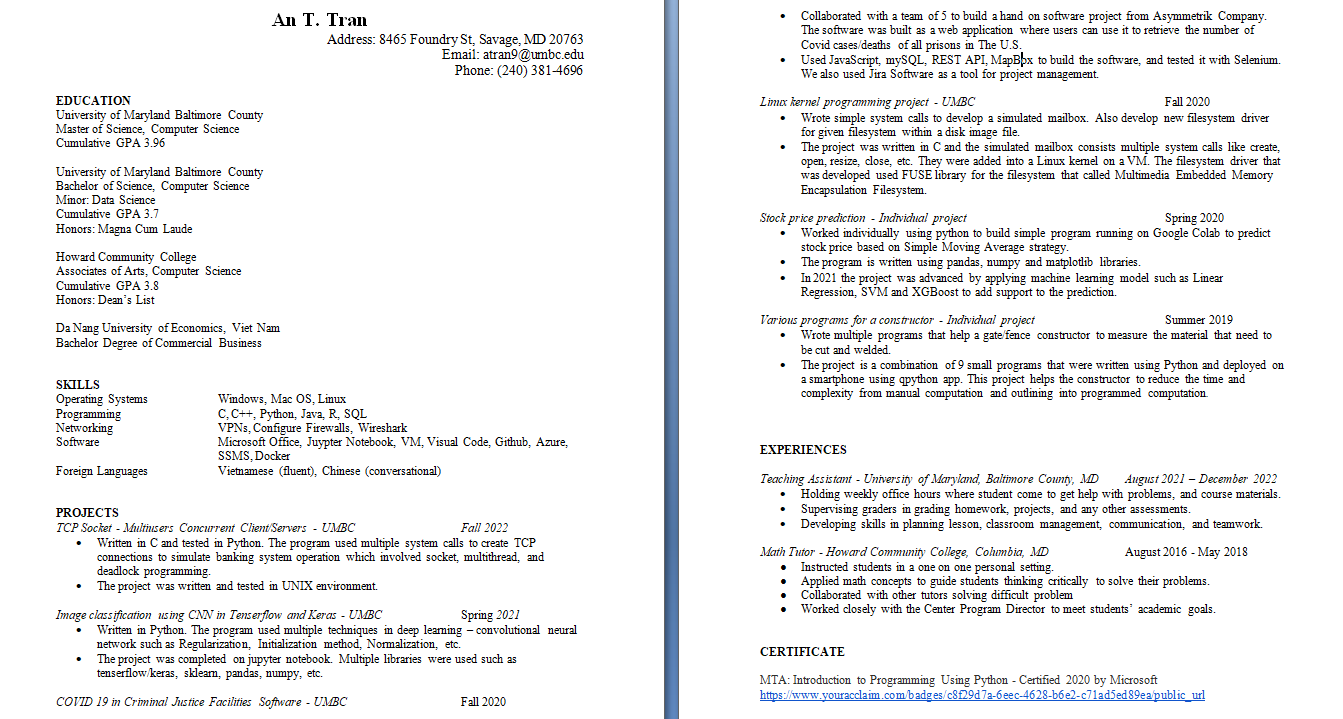
\includegraphics[width=0.8\textwidth]{Original_reume_01.png}
\caption{Original Resume}\label{resume_01}
\end{figure}

\begin{figure}[h]
\centering
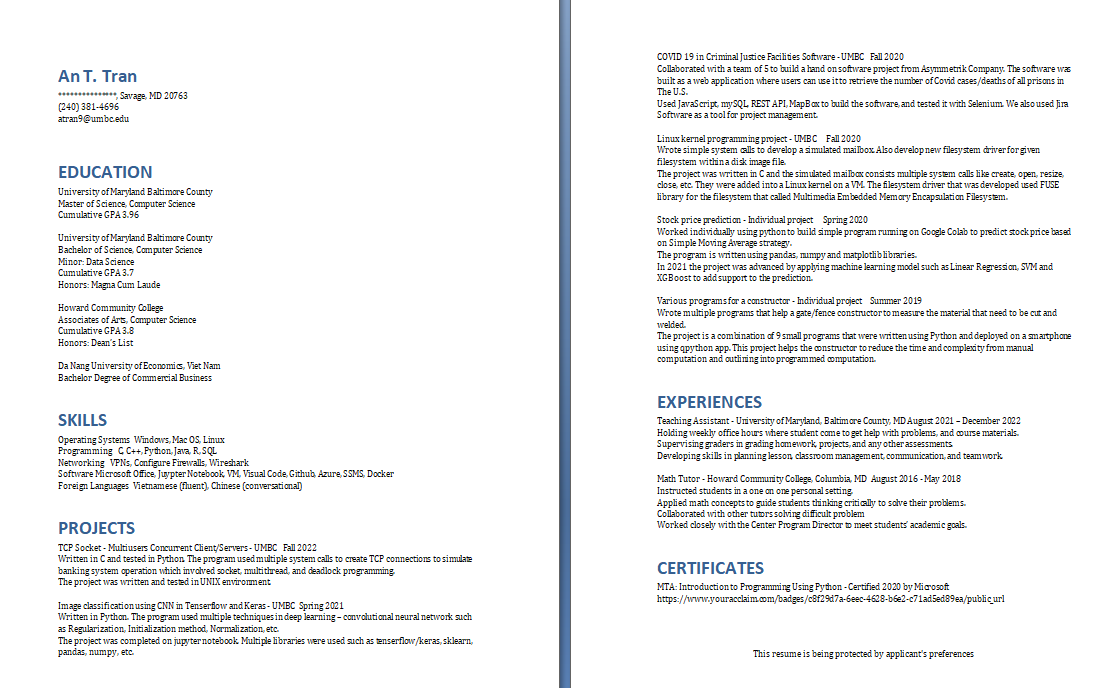
\includegraphics[width=0.8\textwidth]{Risk_01.png}
\caption{Resume after being scraped for risk level 1}\label{risk_01}
\end{figure}

\begin{figure}[h]
\centering
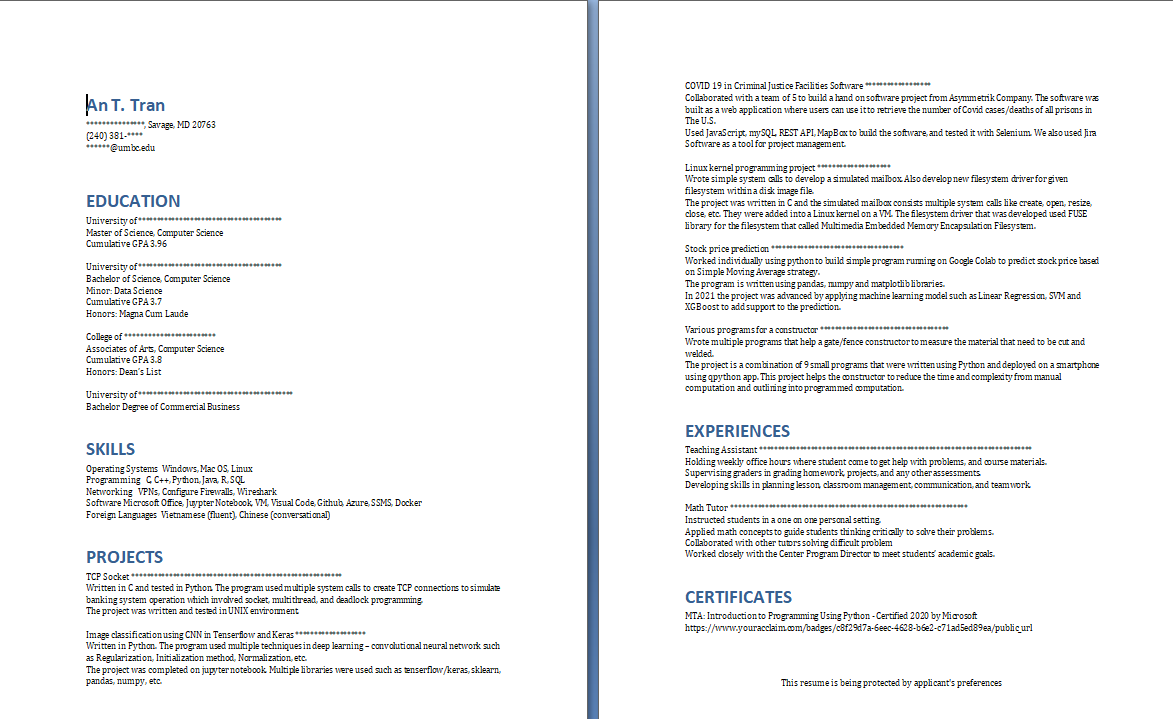
\includegraphics[width=0.8\textwidth]{Risk_05.png}
\caption{Resume after being scraped for risk level 5}\label{risk_05}
\end{figure}


\section{Discussion}

In this project, we collected a list of fake and legitimate companies and stored it as a dataset; we applied qualitative and quantitative analysis and extracted the important features among the determined features. But, our dataset is not a real-world dataset and our analysis can be advanced if we did acquire our results based on the real-world dataset. Also, we applied extensive analysis based on machine learning applications. We applied binary classification and multi-classification models to predict the company's legitimacy and risk level, respectively. Quantitative results also check the model's generalizability by employing the k-fold cross-validation as well. So, we can figure out that the models are robust in the prediction of the risk level and the company's legitimacy.

Scraper covers private information in a way that is less like to reduce an applicant's chance to be recruited. This process is being done by the scraper to not cover information related to applicant capability. For example, for the experience section, the scraper only covers the company name, location, and job time, but does not cover the experience that the applicant gains for that specific position. This helps the applicant remains attractive to the recruiter. Also, as another example, for the education section, the scraper only covers the school name but does not cover other information such as the applicant’s major, GPA, or any other achievement that the applicant has in that school. All of these were done so that applicants still be able to show all their capabilities/skill sets to a recruiter for the position that they are trying to apply for.

Deploying resume scraper helps LinkedIn users to protect their private information from risky companies. However, there is a utility trade-off when a user opts to apply to a company with a resume being scraped. 
\subsubsection{Applicant lost: }
When the user opts to use Scraper and apply to a company that is being detected as a high-risk company, the applicant will use a new protected resume with information covered to apply to the company. Also, the machine learning models have an accuracy of around 90\%, hence there is a chance that the company that the applicant trying to apply to is a legit company but is classified as a risky company. With a resume that has information covered, the applicant may lose the company’s interest in the applicant’s application. For instance, if there is another application that has the same skill sets, experiences, history, and education as an application with a resume being masked, the recruiter is likely to choose the applicant that has an unprotected resume which they can easily locate the applicant's contact information. Therefore, in this case, applicant loses their chance to get hired even if they meet the job’s requirements.
\subsubsection{Recruiter lost:  }
The utility loss happens on the recruiter side when there is a very good candidate that meets everything that the company needs for the hiring position, but the applicant opted to use the resume scraper.  In addition, the company is a legit company but accidentally detected it as a risky company by the machine learning model. This led to the problem that the resume has covered contact information that make the recruiter difficult to contact this good candidate. On the other hand, if this applies also applies to another company that is not detected as a risky company, the other company may easily reach out to the applicant earlier and hire them. Hence, the legit company loses their chance to recruit a good applicant that meets all their requirements for their missing position.
	
At this stage of implementation, this resume scraper can only scrape resumes that are docx-type documents and have a similar format/structure. For future enhancement, we would need to exploit different NLP frameworks that suit best for resume scraping so that it could scrape resumes with all types of structure. The predefined regex would also need to be improved so that it can detect another type of phone number format and address. For instance, currently, the scraper only be able to detect addresses within The U.S.; however, it would need to be able to detect addresses for applicants that live outside of the country and have different address formats. Lastly, the set of keywords needs to be expanded so that it can detect information sections with various headlines. In addition, a variant of the word also needs to be considered. For instance, “Education” needs to be extended to include “EDUCATION, Education, education …”. The expanded list may get long, but this could easily be done by just adding more words to the current keyword list.








\section{Conclusion}
In conclusion, the study sought to address the critical problem of determining the legitimacy of organizations or companies on LinkedIn and projecting their appropriate risk classifications. A robust model was constructed to accurately classify whether a company is legitimate or deceptive by applying Machine Learning techniques, specifically the Decision Trees algorithm.

Additionally, the project's implementation of a scrapper component was a key component. Considering the risk labels projected for each organization, this scrapper was created to extract essential information from resumes. Well-defined policies were created to assure consistency and accuracy in the extraction process. These policies gave instructions on how to assign risk factors to particular resume items and choose which fields needed to be extracted and assessed.

An extensive study was done to identify the elements contributing to the company's legitimacy. This included looking through various resources, analyzing best practices in the business, and taking into account professional viewpoints.  A thorough survey was created, comprising thoughtfully formulated questions that specifically targeted the factors related to the legitimacy of companies. The project team's class and neighborhood received the survey, and an amazing response rate of over 45 participants was obtained. People from different  age groups who actively use LinkedIn for different reasons make up this diverse group. Their insightful suggestions and contributions were thoroughly examined from both quantitative and qualitative  angles. 

The project team was able to identify 11 major features from the survey findings using rigorous quantitative analysis. These features, which included a wide range of properties and indicators, were then incorporated into the dataset. This dataset was used to train and fine-tune the Machine Learning model, allowing for accurate predictions about company legitimacy within the LinkedIn platform.

Overall, this project is a well-executed effort to address the important problem of knowing the legitimacy of companies on LinkedIn. Advanced Machine Learning methods combined with Scraper, data analysis, and policy creation have produced insightful findings and workable solutions for identifying and reducing risk in the professional networking sector. The methodology and findings from this research have the potential to greatly improve the platform's overall trust and security.


\section{Future Scope:-}
\begin{enumerate}
  \item The project has mainly 2 parts.
We developed a machine learning algorithm in the first part of the project to determine whether a company is real or fake. We find out the risks associated with each company with the help of a risk label and this risk label which is predicted, is then inputted into the scrapper.
The second part  of the project is to develop a scraper. We feed the risk labels from the first portion into the scraper, which scrapes resumes depending on the risk labels. This enables us to extract essential information from the resumes for further research.
We need a user-friendly interface that integrates both functionalities to allow smooth coordination between these two elements. We require a front-end system that allows users to interact with the project in a smooth manner, doing functions from a single interface. This interface will make it easier to coordinate and run both portions of the project efficiently.

  \item In terms of the project fields within users' specific LinkedIn profiles, they are assigned a risk level of 2, indicating a moderate level of risk. However, it is important to consider the possibility of certain projects carrying a higher risk. This is particularly relevant when a LinkedIn user showcases both academic and company-related projects they have worked on.

The policy we have established indictates that all projects should be assigned a risk level of 2, without distinguishing between academic and company-related projects. However, this approach raises concerns regarding privacy, as company-related projects cannot be openly disclosed.

To address the above-mentioned issue, we propose the idea of  dividing LinkedIn users into two distinct age groups: users under 20 and users over 20. For users under 20, it is more likely that they have not yet worked with any companies. Therefore, we can assign a risk factor of 2 to the projects section of their profiles. However, for users over 20, there is a higher possibility of having company-related projects. In such cases, we recommend allocating a risk level of 4 to the projects section of their profiles to account for this increased risk.

\end{enumerate}


\section{Members Contribution}

\textbf{Aydin}: Determining and analyzing the features of a legitimate company, qualitative analysis of the features, and extracting the top-5 important factors based on the survey. Generating the risk level for the whole data points by employing a reward function over the features in the dataset. Employing the multi-classification models for predicting the risk level on the dataset and preparing the quantitative results from the model.
Applying the SMOTE on the model for tackling the model imbalance challenge and utilizing the k-fold cross-validation for evaluating the model's robustness.
\\

\textbf{Hrudaya}: Conducted research on risk management approaches and best practices, and gathered relevant information on various risk factors and their potential influence on the candidate's resume during the job application process. Utilizing the research, formulated a systematic framework or methodology to categorize and prioritize risk factors based on the impact. Performed risk assessments and examined historical data to enhance the analysis.
\\

\textbf{Kiran}: I worked on dataset creation. I was primarily involved in data pre-processing and analysis. I performed tasks such as importing the dataset, handling null values, and checking for duplicates. I conducted exploratory data analysis (EDA) by creating visualizations to gain insights. Additionally, I implemented feature selection techniques using correlation analysis. I also played a role in training and evaluating the Decision Trees algorithm for classification. With the help of a decision tree algorithm, I predicted whether the company is real or fake. 

\textbf{An Tran}: I was into the development and implementation of a scraper written in Python. The scraper generates a new version of the resume with the masked information, tailored to the specific company's risk factor criteria. Additionally, discussed the trade-offs involved in using the scraper, both for the applicant and the recruiter, and mentioned areas for future enhancement, such as expanding the capabilities of the scraper to handle different resume formats and improving keyword detection.



























































\section*{References}

\medskip


{
\small


[1] Pandya J, PandiJain G. Detection of Deceptive Accounts Using Machine Learning Algorithm and Deep Neural Network. 2020.

[2] Sahoo PK, Lavanya K. Identification of Malicious Accounts in Facebook. Int J Eng Adv Technol. 2019.

[3] Khaled S, El-Tazi N, Mokhtar HMO. Detecting Fake Accounts on Social Media. In: Proceedings of the 2018 IEEE International Conference on Big Data (Big Data); 2018. p. 3672-3681. doi: 10.1109/BigData.2018.8621913.

[4] Adikari S, Dutta K. Identifying Fake Profiles in LinkedIn. 2020.

[5] Joshi S, Nagariya HG, Dhanotiya N, Jain S. Identifying Fake Profile in Online Social Network: An Overview and Survey. In: Proceedings of the International Conference on Machine Learning; 2020.

[6] [Internet]. Indeed Career Advice. Should You Put Your Address on Your Resume? [cited 2023 May 21]. Available from: https://www.indeed.com/career-advice/resumes-cover-letters/should-you-put-your-address-on-your-resume

[7] [Internet]. Symplicity Corporation. Privacy Policy. [cited 2023 May 21]. Available from: https://www.symplicity.com/compliance/privacy/privacy-policy

[8] [Internet]. Jobscan Blog. Resume Sections: How to Organize and Format Your Resume [cited 2023 May 21]. Available from: https://www.jobscan.co/blog/resume-sections/

[9]  [Internet]. Work - Chron.com. Importance of Personal Information on a Resume [cited 2023 May 21]. Available from: https://work.chron.com/importance-personal-information-resume-20632.html

[10] [Internet]. Python-docx Documentation. Latest Version [cited 2023 May 21]. Available from: https://python-docx.readthedocs.io/en/latest/

[11] [Internet]. SpaCy Documentation. Spacy 101: Everything you need to know [cited 2023 May 21]. Available from: https://spacy.io/usage/spacy-101



%%%%%%%%%%%%%%%%%%%%%%%%%%%%%%%%%%%%%%%%%%%%%%%%%%%%%%%%%%%%


\end{document}